\chapter{完整解答：用十一道问题检查是否学会}
\label{hall:solutions}
本章不是把关键任务转交给读者。每题都给出解答，可以先遮住答案尝试，再逐行核对。

\section{密度相等，为什么还会有电流}
\textbf{题目：}$n_i=n_e=10^{19}$ m$^{-3}$，$u_{ix}=2\times10^4$ m/s，$u_{ex}=-3\times10^4$ m/s，求电荷密度与电流。

\textbf{解：}$\rho_c=e(n_i-n_e)=0$；$J_x=en(u_{ix}-u_{ex})=(1.60218\times10^{-19})(10^{19})(5\times10^4)=8.01\times10^4$ A/m$^2$。电荷密度是两个\emph{数密度}的差，电流是两个\emph{带符号电荷通量}的和。准中性没有要求两个流速相等。

\section{用质心和电流恢复两物种速度}
\textbf{题目：}$m_i/m_e=1836$，$\vct u=0$，$J_z/(en)=10^6$ m/s。

\textbf{解：}解$\vct u=(m_i\vct u_i+m_e\vct u_e)/(m_i+m_e)$与$\vct u_i-\vct u_e=\J/(en)$，得到
\begin{equation}
u_{iz}=\frac{m_e}{m_i+m_e}10^6=544.4\,\mathrm{m/s},\qquad
u_{ez}=-\frac{m_i}{m_i+m_e}10^6=-9.9946\times10^5\,\mathrm{m/s}.
\end{equation}
质心不动不等于粒子不动，也不等于流能为零；此时全部流能都属于两物种的相对漂移。

\section{Hall总功为零，但物种功可以不为零}
\textbf{题目：}$\J=J\hat{\vct z}$、$\B=B\hat{\vct x}$、$u_{iy}=U$，其余速度满足准中性电流关系。求Hall电场和两物种功。

\textbf{解：}$\hat{\vct z}\times\hat{\vct x}=\hat{\vct y}$，故$\E_H=JB\hat{\vct y}/(en)$。因为电流只有$z$分量，$u_{ey}=u_{iy}=U$。离子功$en\vct u_i\cdot\E_H=UJB$，电子功$-en\vct u_e\cdot\E_H=-UJB$，和为零。取$J=10^5$ A/m$^2$、$B=0.02$ T、$U=10^4$ m/s，两者为$\pm2\times10^7$ W/m$^3$。这是欧姆分解中特定电场分量的能量交换，不是两个必然为正的热源。

\section{同样大的压力电场，为什么未必改变磁通}
\textbf{题目：}恒温电子$\Theta_e$不变，$p_e=n\Theta_e$，写出压力项并求旋度。

\textbf{解：}
\begin{equation}
-\frac{\nabla p_e}{en}=-\frac{\Theta_e}{e}\frac{\nabla n}{n}
=-\nabla\left(\frac{\Theta_e}{e}\ln(n/n_\star)\right).
\end{equation}
这里$n_\star$是任意常数参考密度，使对数的自变量无量纲。在光滑单值区域，其旋度为零。它仍可平衡电子压力力、产生电势并改变粒子运动；只是不能单独在Faraday定律中提供感应源。若$\Theta_e$有独立空间梯度，旋度中出现$\nabla\Theta_e\times\nabla n$，必须重新计算。

\section{压缩升温是否就是不可逆加热}
\textbf{题目：}理想单原子标量流体绝热压缩，密度变为原来的2倍，温度变化多少？

\textbf{解：}无热流/耗散时$p/n^{\gamma_s}$沿流不变，$\gamma_s=5/3$。因为$\Theta=p/n$，所以$\Theta/\Theta_0=(n/n_0)^{\gamma_s-1}=2^{2/3}=1.5874$。20 eV升为31.75 eV。理想反向膨胀能回到20 eV，因此这次温升不必伴随熵增加。若要说不可逆，需检查碰撞、黏性、闭合熵或明确粗粒化的贡献。

\section{双束二阶矩为什么容易被叫成“热”}
\textbf{题目：}同一物种有两束各占一半，平均速度为$\pm U\hat{\vct x}$，每束内部各向同性温度能量为$\Theta_0$。求总流、压力和标量温度。

\textbf{解：}总流为零。按中心矩相加，$P_{xx}=n\Theta_0+nmU^2$，$P_{yy}=P_{zz}=n\Theta_0$。因此
\begin{equation}\Theta_{\rm moment}=\frac{\operatorname{tr}\vct P}{3n}=\Theta_0+\frac{mU^2}{3}.\end{equation}
对质子$U=100$ km/s，$m_iU^2/e=104.4$ eV，标量温度多出34.8 eV，但分布仍可保持两束，各束热宽并未增加。若只测$x$方向，额外的方向温度是104.4 eV。两种数不能混写。
\begin{figure}[htbp]\centering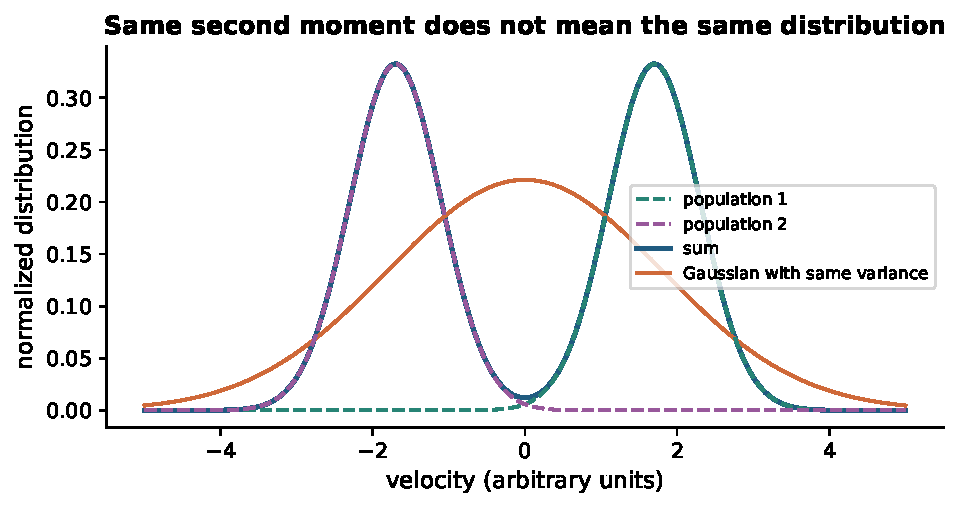
\includegraphics[width=.96\textwidth]{figures/08_multibeam.pdf}
\caption{两个窄高斯束及其和，与同二阶矩的单高斯对比。两者平均速度和方差可以相同，形状与分布熵却不同。图中参数是任意单位的教学输入，不是实验拟合。}\end{figure}

\section{局地各向同性化为什么不增加内能}
\textbf{题目：}只推进$\partial_t\vct P=-\nu(\vct P-p\vct I)$，$p=\operatorname{tr}\vct P/3$，初始$\vct P=\operatorname{diag}(4,1,1)$ Pa。求解。

\textbf{解：}取迹得到$\partial_t\operatorname{tr}\vct P=-\nu(\operatorname{tr}\vct P-3p)=0$，故$p=2$ Pa不变。分别解三个一阶方程：
\begin{equation}P_{xx}=2+2e^{-\nu t},\qquad P_{yy}=P_{zz}=2-e^{-\nu t}.\end{equation}
内能始终为$\operatorname{tr}\vct P/2=3$ J/m$^3$。压强越来越各向同性，不等于总内能越来越大；矩熵可因重排而增加，但要说明定义及闭合来源。

\section{网格缩小一半，Hall显式成本怎样变化}
\textbf{解：}二维格数约增加4倍，时间步若受Hall条件限制缩小为四分之一，同一物理时间需4倍步数，总基础计算量约增加16倍；三维格数增加8倍，总量约增加32倍。通信、隐式求解、缓存和并行效率会改变实际耗时，但这个估计足以说明为什么“再细一倍”不是小代价。仍不能因此省掉必要收敛检查。

\section{一次实验能否证明Hall在X点断线}
\textbf{题目：}二维反平行X点测到$E_z\ne0$，邻近区域测到四极$B_z$，是否可推出$E_z=(\J\times\B)_z/(en)$在X点成立？

\textbf{解：}不能。严格反平行零场X点$\B=0$，Hall项为零；若在二维对称强导场X点仅有$B_z$，$(\J\times\B)_z=J_xB_y-J_yB_x$也为零。非零$E_z$须由电子非理想项平衡。邻近Hall结构与电子内层破冻结是相互关联但不同的问题。

\section{给定密度和磁场，是否已经知道重联热量}
\textbf{解：}给定$B,n$可算每粒子参考磁能$B^2/(2\mu_0n)=m_iV_A^2/2$。实验室例为$6.21\times10^2$ eV每个离子--电子对的参考磁能量级。它没有告诉我们实际释放比例、向外输运比例、流能存储或两物种分配。即使假设全部变成两个物种的均匀标量内能，也只有
\begin{equation}\frac32(\Delta\Theta_i+\Delta\Theta_e)=\frac{B^2}{2\mu_0n},\end{equation}
一条式子约束两个未知温升。还需独立能量方程和机制，不能凭Hall项补一个固定2:1比例。

\section{一页自检：不用背诵，也应该能解释}
读完后应能连贯说明：Hall项来自电子--离子速度差；准中性允许有限电流；取矩是恒等操作而闭合是额外模型；电子惯性小不小取决于层厚、频率和速度；磁冻结应指明跟哪种速度；X点电场必须按分量检查；压力功、温升与不可逆热化不同；$d_i,\rho_i,\rho_s,\lambda_D$各有含义；一个全局大$S$不能保证局地MHD成立；一张四极图或一条相近重联率不足以证明闭合与加热全部正确。

如果其中某项仍只能复述结论，建议回到相应章节重算一个数字例。真正的掌握不是记住更多模型名字，而是能在新参数下重新选择近似，并明确模型预测的边界。
